\subsection{Pseudodynamic minimaps}
\label{sec:method}


A recording is a sequence of samples $p_i = (x_i, y_i, t_i, c_i, \mathbf{s}_i)$, with position,
timestamp, a contact flag and a vector of per-sample signals. Only segments with contact at both
ends are drawn.

\paragraph{Geometry.} Contact points are fitted to a $512 \times 512$ canvas with a $20$~px margin,
preserving aspect ratio, and drawn as $4$~px line segments with $3\times$ supersampling followed by
Lanczos downsampling. A second geometry fixes the scale per task in device units instead of fitting
it per recording, so that absolute size is preserved across participants; its reference extent is
taken over every recording of that task without labels, which makes that arm transductive.
Every number reported in this paper comes from the canvas-fitted geometry; the fixed-scale arm is
kept only because it was declared, and it is never the arm a result rests on.

\paragraph{Colour.} For a chosen signal $s$ and segment $i$, the value is the mean of its endpoints,
$\bar{s}_i = (s_i + s_{i+1})/2$, normalised \emph{within the recording} by its own $5$th and $95$th
percentiles,
\begin{equation}
\tilde{s}_i = \mathrm{clip}\!\left(\frac{\bar{s}_i - q_{05}(s)}{q_{95}(s) - q_{05}(s)},\, 0,\, 1\right),
\end{equation}
and mapped affinely to a channel range $[30, 220]$. Speed is $\log(1+v)$ before normalisation;
azimuth is centred circularly before normalisation. Three signals can be assigned to the three
channels at once, giving the nine encodings we evaluate: the bare trace, four single-signal
minimaps (\textbf{S}peed, \textbf{P}ressure, \textbf{A}ltitude, a\textbf{Z}imuth) and four
triples (\cref{fig:examples}).

\begin{figure}[t]
\begin{center}
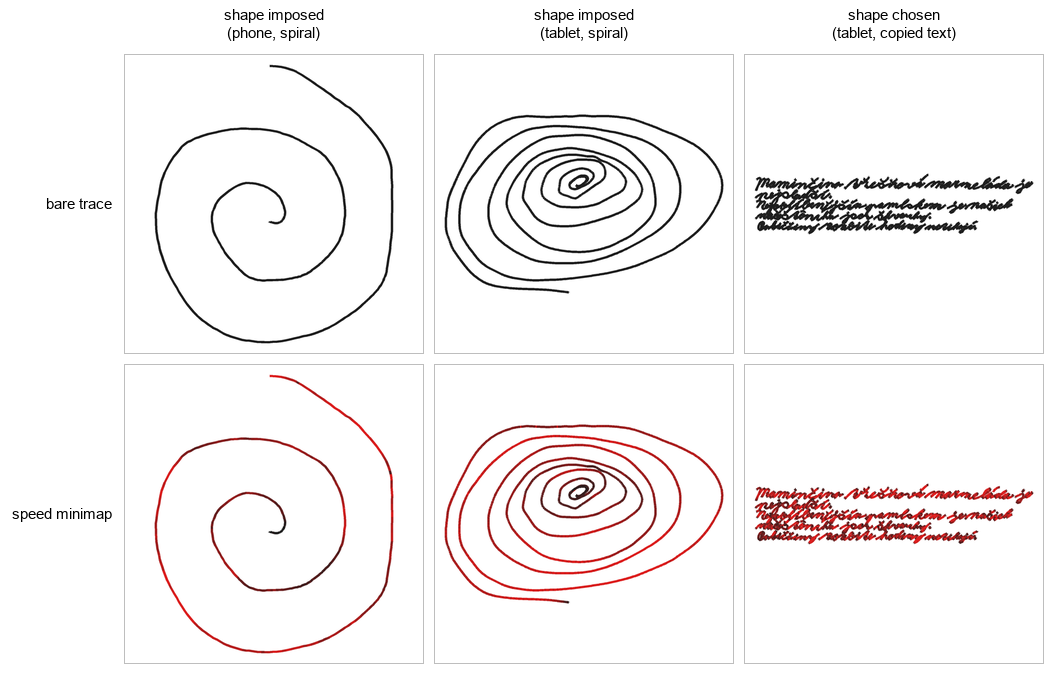
\includegraphics[width=\columnwidth]{figures/examples.png}
\end{center}
\caption{The same encoding on the two task regimes of \cref{sec:tasks}, read from recordings the
experiments actually used. Left and centre: the task prescribes the figure, so the bare trace is
nearly the same for everyone and what differs is the execution the colour carries. Right: a copied
text, where the produced shape already carries most of what distinguishes one recording from
another, and where the square canvas shrinks a wide multi-line page into a strip. No participant is
identified and no panel was chosen for its appearance.}
\label{fig:examples}
\end{figure}

Two properties matter for the argument. The normalisation uses no statistic of the cohort and no
label, so nothing about the class distribution can enter the image; and the mapping is
\emph{positional}, the only part of the pipeline that records where along the trace a value
occurred, which is what the controls of \cref{sec:results-controls} test directly.

\paragraph{Descriptor and model.} Unless stated otherwise, images are described by Local Phase
Quantisation (LPQ) \citep{ojansivu2008lpq} on each channel ($64 \times 64$, $5\times 5$ window,
$256$ bins per channel, $768$ dimensions, square-root transformed) and classified by a support
vector machine. A frozen ImageNet ResNet18 \citep{he2016resnet} with an $\ell_2$-regularised
logistic head is the second descriptor over the identical images, which separates the encoding's
contribution from the descriptor's.

